
%%%%%%%%%%%%%%%%%%%%%%% file typeinst.tex %%%%%%%%%%%%%%%%%%%%%%%%%
%
% This is the LaTeX source for the instructions to authors using
% the LaTeX document class 'llncs.cls' for contributions to
% the Lecture Notes in Computer Sciences series.
% http://www.springer.com/lncs       Springer Heidelberg 2006/05/04
%
% It may be used as a template for your own input - copy it
% to a new file with a new name and use it as the basis
% for your article.
%
% NB: the document class 'llncs' has its own and detailed documentation,  see
% ftp://ftp.springer.de/data/pubftp/pub/tex/latex/llncs/latex2e/llncsdoc.pdf
%
%%%%%%%%%%%%%%%%%%%%%%%%%%%%%%%%%%%%%%%%%%%%%%%%%%%%%%%%%%%%%%%%%%%


\documentclass[runningheads, a4paper]{llncs}



\usepackage[linesnumbered,ruled]{algorithm2e}

\usepackage[margin=0.5in]{geometry}
\usepackage{amssymb}
\setcounter{tocdepth}{3}
\usepackage{graphicx}
\usepackage{amssymb}% http://ctan.org/pkg/amssymb
\usepackage{pifont}% http://ctan.org/pkg/pifont
\newcommand{\cmark}{\ding{51}}%
\newcommand{\xmark}{\ding{55}}%

\usepackage{floatrow}
% Table float box with bottom caption, box width adjusted to content
\newfloatcommand{capbtabbox}{table}[][\FBwidth]
\usepackage{caption}
\usepackage{subcaption}
\captionsetup{compatibility=false}

\usepackage{url} % for bibliograpy links
\urlstyle{same}  % (for bibliography links
\usepackage{float} % To force image to stand still

\usepackage{amsmath,amssymb}

\usepackage{color}

\usepackage{array}
\newcolumntype{P}[1]{>{\centering\arraybackslash}p{#1}}





\usepackage{xcolor} % Colors

\usepackage{tikz}
\usepackage{keyval}
\usepackage{pgfplots} % Bar charts

\usepgfplotslibrary{groupplots}

%\usepackage{groupplots}
%\usepgfplotslibrary{groupplots}
\pgfplotsset{compat=newest}


%
% Define bar chart colors
%
\definecolor{bblue}{HTML}{4F81BD}
\definecolor{rred}{HTML}{C0504D}
\definecolor{ggreen}{HTML}{9BBB59}
\definecolor{ppurple}{HTML}{9F4C7C}


\usepackage{amssymb}
\setcounter{tocdepth}{3}
\usepackage{graphicx}

\newcommand{\keywords}[1]{\par\addvspace\baselineskip
    \noindent\keywordname\enspace\ignorespaces#1}







%%%%%%%%%%%%%%%%%%%%%%%%%%%%%%%%%%%%%%%%%
%           START OF COMMANDS
%%%%%%%%%%%%%%%%%%%%%%%%%%%%%%%%%%%%%%%%%


%%%%%%%%%%%%%%%%%%%%%%%%%%%%%%%%%
% Save results to be later used in addBarPlotResults
% #1: Train Small
% #2: Train Big
% #3: Train All
% #4: Test
%%%%%%%%%%%%%%%%%%%%%%%%%%%%%%%%%
\newcommand{\saveResultsFirst}[4]{
    \def\TrainSmallFirst{#1}%
    \def\TrainBigFirst{#2}%
    \def\TrainAllFirst{#3}%
    \def\TestFirst{#4}%
}

%%%%%%%%%%%%%%%%%%%%%%%%%%%%%%%%%
% Save results to be later used in addBarPlotResults
% #1: Train Small
% #2: Train Big
% #3: Train All
% #4: Test
%%%%%%%%%%%%%%%%%%%%%%%%%%%%%%%%%
\newcommand{\saveResultsSecond}[4]{
    \def\TrainSmallSecond{#1}%
    \def\TrainBigSecond{#2}%
    \def\TrainAllSecond{#3}%
    \def\TestSecond{#4}%
}

%%%%%%%%%%%%%%%%%%%%%%%%%%%%%%%%%
% Adds Results to Bars labeled by #1, #2
%
% Label #1 is used for saveResultsFirst
% Label #2 is used for saveResultsSecond
%
%%%%%%%%%%%%%%%%%%%%%%%%%%%%%%%%%
\newcommand{\addBarPlotResults}[2]{
    % TRAINING |w| < C    
    \addplot[style={bblue, fill=bblue, mark=none}]
    coordinates 
    {
        (#1,  \TrainSmallFirst)
        (#2,  \TrainSmallSecond)
    };
    
    % TRAINING |w| > C
    \addplot[style={rred, fill=rred, mark=none}]
    coordinates 
    {
        (#1,  \TrainBigFirst)
        (#2,  \TrainBigSecond)
    };
    
    % TRAINING ALL
    \addplot[style={ggreen, fill=ggreen, mark=none}]
    coordinates 
    {
        (#1,  \TrainAllFirst)
        (#2,  \TrainAllSecond)
    };
    
    % TESTING
    \addplot[style={ppurple, fill=ppurple, mark=none}]
    coordinates 
    {
        (#1,  \TestFirst)
        (#2,  \TestSecond)
    };
}



%%%%%%%%%%%%%%%%%%%%%%%%%%%%%%%%%
% Adds needed style to pgfplot
%%%%%%%%%%%%%%%%%%%%%%%%%%%%%%%%%
\newcommand{\setPlotStyle}[0]{
    \pgfplotsset{xticklabel style={text width=2em, align=center}}
}

%%%%%%%%%%%%%%%%%%%%%%%%%%%%%%%%%
% Starts groupplot with given style
%%%%%%%%%%%%%%%%%%%%%%%%%%%%%%%%%
\newcommand{\beginGroupPlot}[0]{
    \begin{groupplot}[
        group style={group size= 2 by 2,  vertical sep=50pt},
        height = 5.5cm, 
        ybar=4*\pgflinewidth, 
        ymin=0, 
        ymax=1,
        width  = 0.37*\textwidth, 
        enlarge x limits={abs=0.85cm}, 
        major x tick style = transparent, 
        ymajorgrids = true, 
        symbolic x coords={
            C=4,
            C=4 Q=3,
            C=4 Q=4,
            C=4 Q=5,
            C=4 Q=6,
            C=4 Q=7,
            C=4 Q=8,
            C=4 Q=9,
            C=4 Q=10,
            C=4 Q=11,
            C=4 Q=12,
            C=4 Q=13,
            C=4 Q=14,
            C=4 Q=15,
            C=5,
            C=5 Q=3,
            C=5 Q=4,
            C=5 Q=5,
            C=5 Q=6,
            C=5 Q=7,
            C=5 Q=8,
            C=5 Q=9,
            C=5 Q=10,
            C=5 Q=11,
            C=5 Q=12,
            C=5 Q=13,
            C=5 Q=14,
            C=5 Q=15
        },
        xtick = data, 
        scaled y ticks = false, 
        legend cell align=center, 
        legend columns=1,
        legend style={
            at={(1.45, 0.45)}, 
            anchor=north,
        }
        ]
    }%beginGroupPlot
    
    %%%%%%%%%%%%%%%%%%%%%%%%%%%%%%%%%
    % Sets legends for Bar plot
    %%%%%%%%%%%%%%%%%%%%%%%%%%%%%%%%%
    \newcommand{\setPlotLegend}[0]{
        \legend{Training $|w|<C$,  Training $|w|>C$,  Training All,  Testing}
    }
    
    %%%%%%%%%%%%%%%%%%%%%%%%%%%%%%%%%%%%%%%%%
    %           END OF COMMANDS
    %%%%%%%%%%%%%%%%%%%%%%%%%%%%%%%%%%%%%%%%%
    
    
    
    
\begin{document}
    
\mainmatter  % start of an individual contribution

\title{Krotkodystansowy Komiwojazer \\ Bottleneck Traveling Salesman Problem}

% a short form should be given in case it is too long for the running head
\titlerunning{Bottleneck TSP}

\author{Jakub Ciecierski \and Wojcik Lukasz \\ 
    \textit{Warsaw University of Technology, \\
        Faculty of Mathematics and Information Science.}}
%

\authorrunning{Bottleneck TSP}

\toctitle{Bottleneck TSP}
\tocauthor{Methodology}
\maketitle
        
        
        
        
        
%---------------------------------------------------------------------
%---------------------------------------------------------------------
%---------------------------------------------------------------------
\section{Introduction}
In standard Traveling Salesman Problem (TSP), we are interesting in finding the Hamiltonian cycle with smallest sum of weights. The Bottleneck Traveling Salesman Problem (BTSP) focuses only on minimizing the cost of the heaviest weighted edge, called a bottleneck. Let $b$ denote a function that outputs the bottleneck value for given graph.

This paper introduces the reader to the 3-approximation algorithm for BTSP for complete undirected graphs with cost function satisfying triangle inequality. The algorithm runs in linear time. Authors provide the pseudo code for the algorithm together with proof of approximation ratio property and time complexity analysis.

The paper starts with preliminary definitions important to problem description. Further, approximation algorithm for classical TSP problem is presented for reference point of view. Then, the BTSP algorithm is presented and analyzed. The paper ends with input and output format for the problem implementation.

%---------------------------------------------------------------------
%---------------------------------------------------------------------
%---------------------------------------------------------------------
\section{Preliminaries}

\subsection{Triangle inequality}

The cost function c satisfies the \textbf{triangle inequality} if, for all vertices $u,v,w \in V$

\begin{center}
    $c(u,v)\leq c(u,v) + c(v,w)$
\end{center}

It means that adding intermediate steps between some vertices will never decrease the cost.

%---------------------------------------------------------------------
%---------------------------------------------------------------------
\subsection{TSP}

\textbf{Traveling salesman problem} in a given graph is asking for a Hamiltonian cycle with the smallest possible sum of weights.

\subsubsection{Aproximation algorithm.}
To find TSP cycle we have to find a \textbf{minimum spanning tree (MST)} first. Sum of weights of MST gives us a lower bound on cost of optimal TSP tour. It also will be used to create a tour whose cost is no more than twice that of the minimum spanning tree's wight (having that it satisfies the triangle inequality). We assume that an input for our algorithm is a complete, undirected graph with vertex r as a root and c satisfies the triangle inequality.
        
        
\begin{algorithm}[H]
    \SetKwInOut{Input}{Input}
    \SetKwInOut{Output}{Output}
    \Input{complete, undirected graph $G$, cost function $c$ satisfying triangle inequality. }
    \Output{Hamiltonian cycle H}
    select a vertex $r \in G.V$ to be a root vertex \\
    
    compute a minimum spanning tree T for G from root r using MST-PRIM(G,c,r) \\
    
    let H be a list of vertices, ordered according to when they are first visited in a preorder tree walk of T \\
    
    return the hamiltonian cycle H \\
    
    %  \underline{function HILL-CLIMBING-IMPROVED} $(s, n)$\;
    %  $i = 0$ \\
    %  $current = s$ \\
    %  \While{$i < n$}
    %  {
    %  	$neighbor$ $\gets$ randomly generated state, different than $current$ \\
    
    %	\If{OBJ-FUNCTION[neighbor] $\geq$ OBJ-FUNCTION[current]}
    %	{
    %		$current$ $\gets$ $neighbor$
    %	}
    
    % }
    \caption{Approx-TSP-Tour}
    \label{algo:hc_improved}
\end{algorithm}
        
        
%---------------------------------------------------------------------
%---------------------------------------------------------------------
\section{Bottleneck TSP}

Solving Bottleneck Traveling Salesman Problem is equivalent to finding a Hamiltonian cycle in which the heaviest edge weight is as small as possible. The heaviest edge weight that remains in the cycle is called a bottleneck. The following presents an 3-approximation algorithm for solving BTSP problem. The approximation ratio states that the resulting Hamiltonian cycle can have a bottleneck with cost at most 3 times greater than the optimal solution.

The idea for the algorithm is to compute a Minimum Bottleneck Spanning Tree (MBST) and construct a Hamiltonian cycle by taking a full walk of the tree and skipping no more than 2 consecutive intermediate vertices.

Let us first consider the algorithm for constructing MBST. As input, we provide a connected and undirected graph together with a cost function defining weights for all edges. The output contains a spanning tree with minimum heaviest weight, hence a MBST. The full pseudo code is presented in algorithm~\ref{alg:mbst}. First, we compute the median weight and partition the graph around it. The edges with weight greater than median are put to set $A$, the remaining edges are in $B$. Then we check whether $B$ contains a single connected component and spans all vertices, if yes then we can simply considered edges in $A$ as rejected and continue removing heavy edges from $B$ by recursively calling a graph constructed by the set of edges $B$. In the case when the partitioning divided $B$ into multiple connected components we contract the components to create a new connected graph. Each of the connected components of $B$ are contracted into a single super vertex. Then the edges of $A$ are used to connected these super vertices. The process is repeated until we end up with two super vertices which we can be connected by the edge with smallest weight.
The contracting process is presented in algorithm~\ref{alg:mbst_contract}
        
\begin{algorithm}[H]
    \SetKwInOut{Input}{Input}
    \SetKwInOut{Output}{Output}
    \Input{
        $G(V,E)$ - Connected, undirected graph, where $V$ is the set of vertices and $E$ is the set of edges \\
        $c$ - Cost function. $c: E -> N$
    }
    \Output{$T$ - Minimum Bottleneck Spanning Tree}
    
    \If{$|G.E|$ = 1}{return $G$}
    
    $m = computeMedianWeight(G)$ \\
    $A = \{e : {e {\in G.E}} \land c(e) > m \}$. Set of edges with weight greater than $m$ \\
    $B = \{e : {e{\in G.E}} \land c(e) \leq m \}$. Set of edges with weight smaller or equal to $m$ \\
	\If{$|B| == |G.E|$}
        {
            Take one edge from B and move it to set A.\\			
        }     
    
    $F =$ Forest(B) \\
    
    \If{$|F|=1$ and spans all vertices}{  	
        
        $G^{'}.V = G.V$ \\
        $G^{'}.E = B$ \\
        return MBST$(G^{'})$
    }
    \Else {
        $G^{'}$ = MBST-Contract$(F, A)$
        
        return $F$ $\cup$ MBST($G^{'}$)
    }
    
    \caption{MBST(G, c)}
    \label{alg:mbst}
\end{algorithm}



\begin{algorithm}[H]
    \SetKwInOut{Input}{Input}
    \SetKwInOut{Output}{Output}
    \Input{
        $F$ - Forest,
        $A$ - Set of edges
    }
    \Output{$G$ - Connected graph}
    
    $V_{F} = $ A single super vertex is created for each connected component of $F$. Each such vertex corresponds to its connected component. \\
    $V = $ Missing Vertices in $F$. Vertices in $A$ but not in $F$ \\
    
    $E_{F}$ = Edges from $A$ that connect the connected components of $F$\\
    $E$ = Edges from $A$ to missing vertices in $F$ \\
    
    $G.V = $ $V_{F} \cup V $ \\
    $G.E = $ $E_{F} \cup E $
    
    return $G$
    
    \caption{MBST-Contract(F, A)}
    \label{alg:mbst_contract}
\end{algorithm}

Finally, the pseudo code for 3-approximation BTSP is shown in algorithm~\ref{alg:btsp}. As promised, we first construct MBST, and then compute a full walk of the tree and skip at most 2 constitutive intermediate vertices.

\begin{algorithm}[H]
    \SetKwInOut{Input}{Input}
    \SetKwInOut{Output}{Output}
    \Input{
        $G(V,E)$ - complete, undirected graph, where $V$ is the set of vertices and $E$ is the set of edges \\
        $r$ - root $r \in G.V$ \\
        $c$ - Cost function satisfying triangle inequality. $c: E -> N$
    }
    \Output{$H$ - Hamiltonian cycle}
    $T = $ MBST$(G,c)$ \\
    
    $H = $ Hamiltonian cycle obtained by listing vertices in T such that the distance (in T) between to adjacent vertices (in the sequence) is not greater than 3. \\
    
    \While{sequence does not contain all vertices}
    {
		\For{number of children of current node}
		{
			\If{child was visited}
			{
				do nothing
			}
			\Else
			{
				currentNode = child\\
				currentDistance +=1\\
				\If{currentDistance == 3}
				{
					mark current node as visited \\
					add current node to H\\
					currentDistance = 0 \\
				}
			}
		}
		\If{all children were visited or there is no child}
		{
			\If{currentNode was not visited}
			{
				change it's status to visited\\
				add currentNode to H\\
				currentDistance = 0;
			}
			if (currentNode != R)		
			{
				currentNode = currentNode.Parent;
				currentDist++;
			}
		}		
		
    }
    
    return $H$
    \caption{BTSP-Approx(G,c)}
    \label{alg:btsp}
\end{algorithm}

%---------------------------------------------------------------------
%---------------------------------------------------------------------
%---------------------------------------------------------------------
\section{Analysis}

%---------------------------------------------------------------------
%---------------------------------------------------------------------
\subsection{Correctness}

First, let us consider minimum spanning tree $T$ and bottleneck spanning tree $T_{b}$ of the same graph $G$. It can be easily shown that $T$ is also a bottleneck spanning tree since discarding the heaviest weighed edge, contributes to the smallest sum of weights in the spanning tree. However a bottleneck spanning tree is not necessarily minimum spanning tree. Although, if the heaviest edge in $T$ has weight $w$, then the bottleneck in $T_{b}$ is at most $w$.

\begin{theorem} \label{thm:mbst}
    MBST finds Minimum Bottleneck Spanning Tree
\end{theorem}

\textbf {Proof of Theorem~\ref{thm:mbst}:}

After each iteration, the graph is half divided around the median of weights of edges. Suppose that $B$ is the set of edges with weights smaller or equal to median and $A$ the set of remaining edges. If $B$ is a single connected component then the edges in $A$ are considered to be too heavy and thus rejected. In this simply case we can see that if $B$ remains connected without some of the heaviest edges, the algorithm will successfully remove them. However, if after partitioning, $B$ contains multiple connected components, the graph has to be contracted. The algorithm contracts each of the connected components of $B$ into a single super vertex so that the input of recursive call is a connected graph.

\begin{theorem} \label{thm:tree_seq}
    Let $T$ be a tree rooted at $r$ with at least two vertices. We can list all the vertices of $T$ in sequence such that the distance (in $T$) between two adjacent vertices(in the sequence) is not greater than 3. First and last vertices are considered to be adjacent. The vertex following $r$(in sequence) must be adjacent (in $T$) to $r$.
\end{theorem}

\textbf {Proof of Theorem~\ref{thm:tree_seq}:}

The proof is by induction on number of vertices $n$. \\
\textbf{Basis:} $n=2$ Thus the property of theorem~\ref{thm:tree_seq} obviously holds.\\
\textbf{Induction:} Assume that tree has $n$ vertices and there exists a sequence satisfying the property. Let us show that the property also holds for $n+1$ vertices.
TODO

\begin{theorem} \label{thm:btsp}
    BTSP-Approx is a 3-approximation of BTSP problem.
\end{theorem}

\textbf {Proof of Theorem~\ref{thm:btsp}}\\
        
We receive MBST $T$ by removing heaviest of edges. Also, $T$ is essentially obtained by removing a single heaviest edge from a cycle. Thus MBST provides a lower bound solution for optimal Hamiltonian cycle $H^*$ in the BTSP problem.
\begin{center}
    $b(T) \leq b(H^*)$
\end{center}

In our BTSP-Approx algorithm we obtained a Hamiltonian cycle $H$ by traversing the graph by skipping at most 2 vertices in the full walk of $T$. Considering that the cost function $c$ satisfies triangle inequality then we get:

\begin{center}
    $b(H) \leq 3b(T)$
\end{center}

Combining the two equations we finally get:

\begin{center}
    $b(H) \leq 3b(H^*)$
\end{center}
Which  ends our proof.
The figure~\ref{fig:3approx_proof} shows the idea of skipping. By triangle inequality we get $c(B,C) \leq 3 * 5 = 15$
\begin{figure}[H]
    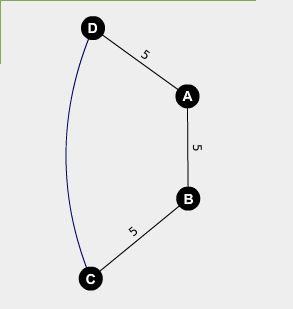
\includegraphics[width=0.30\textwidth]{res/3approx_proof.png}
    \caption{Figure presents the idea of proofing the 3-approximation property of BTSP-Approx.}
    \label{fig:3approx_proof}
\end{figure}

%---------------------------------------------------------------------
%---------------------------------------------------------------------
\subsection{Time Complexity}
\subsubsection{Algoritm~\ref{alg:mbst} MBST}
runs in $O(V+E)$ time. Proof:

\begin{itemize}
  \item lines 1-2 $O(1)$ 
  \item line 4 $O(E)$ - median selection algorithm \cite{cormen_9}
  \item lines 5-6 $O(E)$ - linear search of edges
  \item line 7 $O(E)$ - check if number of edges  in both sets is equal (linear)
  \item line 8 $O(1)$
  \item line 10 $O(E+V)$ (O(n)) - every edge is considered twice and every node is processed once
  \item line 11 $O(V)$ - check if size of forest is equal to 1 and if number of vertices in forest is equal to number of vertices in input graph (linear)
  \item line 12 $O(V)$ - copy V vertices from G'.V
  \item line 13 $O(E)$ - copy E edges from B to G'.E
  \item line 17 $O(V+E)$ - complexity of algorithm~\ref{alg:mbst_contract} MBST-Contract
\end{itemize}

In each recursive call we have 2 times less edges than in the calling function so complexity will also be 2 times smaller. Sum of costs of all calls of this function (including initial one will be not bigger than $O(2V + 2E) == O(V+E)$

\textbf{Sum} - $O(V + E)$
\subsubsection{Algoritm~\ref{alg:mbst_contract} MBST-Contract}
runs in $O(V+E)$ time. Proof:

\begin{itemize}
    \item line 1 $O(V)$ - linear search of connected components in F
    \item line 2 $O(V)$ - linear search of vertices not in F
    \item line 3 $O(E)$ - linear search of edges connecting vertices in F
    \item line 4 $O(E)$ - linear search of edges connected to vertices not in F
    \item line 5 $O(V)$ - linear copy of vertices
    \item line 6 $O(E)$ - linear copy of edges
\end{itemize}

\textbf{Sum} - $O(V + E)$

\subsubsection{Algorithm~\ref{alg:btsp} BTSP}
runs in $O(V+E)$ time. Proof:
TODO
%---------------------------------------------------------------------
%---------------------------------------------------------------------
%---------------------------------------------------------------------
\section{Input/Output}
The input graph must be complete, undirected and the cost function of weights must satisfy triangle inequality. We propose the input graph to consist of vertices with given coordinates in two dimensional euclidean space. Thus each vertex will represent a node, or city and its $(x,y)$ coordinates will represent its position in the map. The cost function will be simply the euclidean distance between two vertices, which satisfies the triangle inequality, as well as the completeness of the graph. Each vertex will given an id number, where the first vertex is the root or the starting point.

The output cycle, will also be a list of vertices with their $(x,y)$ coordinates, although in this case the position in the sequence matters. The vertices will be listed in top down fashion where each of the adjacent vertices are considered to be connected. The first (root) and the last are also connected. The sample files of the explained format are presented in figure~\ref{fig:io}.

\begin{figure}[H]
    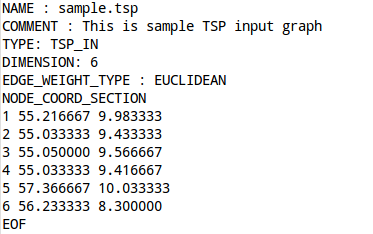
\includegraphics[width=0.4\textwidth]{res/tsp_input.png}
    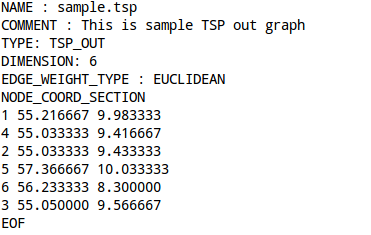
\includegraphics[width=0.4\textwidth]{res/tsp_out.png}
    
    \caption{Example of input (left) and output (right) files}
    \label{fig:io}
\end{figure}


\begin{thebibliography}{4}
    
    \bibitem{cormen} Cormen, Thomas H.; Leiserson, Charles E.; Rivest, Ronald L.; Stein, Clifford (2009) [1990]. Introduction to Algorithms (3rd ed.). MIT Press and McGraw-Hill. ISBN 0-262-03384-4.
    
    \bibitem{cormen_9} Thomas H. Cormen, Charles E. Leiserson, Ronald L. Rivest, and Clifford Stein. Introduction to Algorithms, Second Edition. MIT Press and McGraw-Hill, 2001. ISBN 0-262-03293-7. Chapter 9: Medians and Order Statistics, pp. 183–196. Section 14.1: Dynamic order statistics, pp. 302–308.
\end{thebibliography}
        
\end{document}
